\section{Methods}

Here we describe the rank epistasis algorithm, as well as a proof-of-concept experiment to test its efficacy and an illustrative comparison between rank epistasis and traditional metrics. 

\subsection{Rank Epistasis Algorithm}
To evaluate a target locus with rank epistasis, do the following: 

\begin{enumerate}

\item \textit{Choose a reference genome.} In digital systems, this may be the maximally performing organism; in biological systems, this may be the wild type. This reference genome will be used as the baseline for creating one- and two-step mutants, so it should be a genome representative of the general population of interest.

\item \textit{For each site in the reference genome, measure the fitness effect of each one-step mutant across all non-target loci.}  For large genomes (or limited testing) it may be more tractable to sample a fixed sub-set of mutations. This step will give us a baseline for evaluating how single mutations at each site affect fitness of the entire genome.

\item \textit{Rank the single-step mutants by fitness.} The resultant list is the \textbf{reference ranking}. Ties are broken by taking the average rank of the tied candidates. 

\item \textit{Apply a mutation to the target locus and repeat step 2.} This generates the set of all two-step mutants which include the target locus, so that we can evaluate how a mutation at that locus interacts with the existing mutations at all other loci.

\item \textit{Rank the two-step mutants by fitness.} The resultant list is the \textbf{target ranking}. Ties are again broken by averaging across rank. This creates a ranking which reflects the relative fitness of all two-step mutants where one of the mutations is at the target locus, so that we may compare it to the relative fitness of one-step mutants \textit{without} the target locus.

\item \textit{Calculate Wilcoxon Signed-Rank Sum between the two rankings.} Using the reference and target rankings as ranked lists paired by reference locus, calculate the Wilcoxon Signed-Rank Sum of the two lists. The Wilcoxon statistic, here designated $\omega$, is used as the final measure of epistasis for the target locus, referred to as that locus's \textbf{epistatic load}. This $\omega$ reflects the difference between the two ranked lists of genomes: one containing all single-step mutants \textit{except} at a single site, and one containing all two-step mutants which \textit{include} that site. The difference between how these genomes are ranked reflects how much the mutation at the target site perturbs the fitness effects of other genes in the genotype.

\item \textit{Repeat step 2-6 for all distinct possible mutations at the target locus.} We can then average $\omega$ across all mutations to measure how heavily the target locus interacts with other loci in the genome.

\end{enumerate}

This procedure allows us to calculate the \textit{epistatic load} at a single locus, without needing to first make a baseline assumption about the type of interactions among loci.  
This per-locus epistasis metric can be aggregated to measure epistasis across a whole organism (as is common in other epistatic measurements \citep{elena_test_1997, franklin_mapping_2019}), or for a single locus across a population at a point in time. 

\subsection{Comparisons of Baseline Assumptions}

Current metrics for epistasis take a baseline assumption of either additivity or multiplicativity; however, choosing the wrong metric will detect epistasis where none exists. Further, in genomes with both additive and multiplicative components, it is impossible to choose a correct metric as the assumption will be at least partially incorrect. Therefore, we created a mixed additive and muliplicative model genome to evaluate rank epistasis compared to traditional models with baseline assumptions.

\begin{figure}
    \centering
    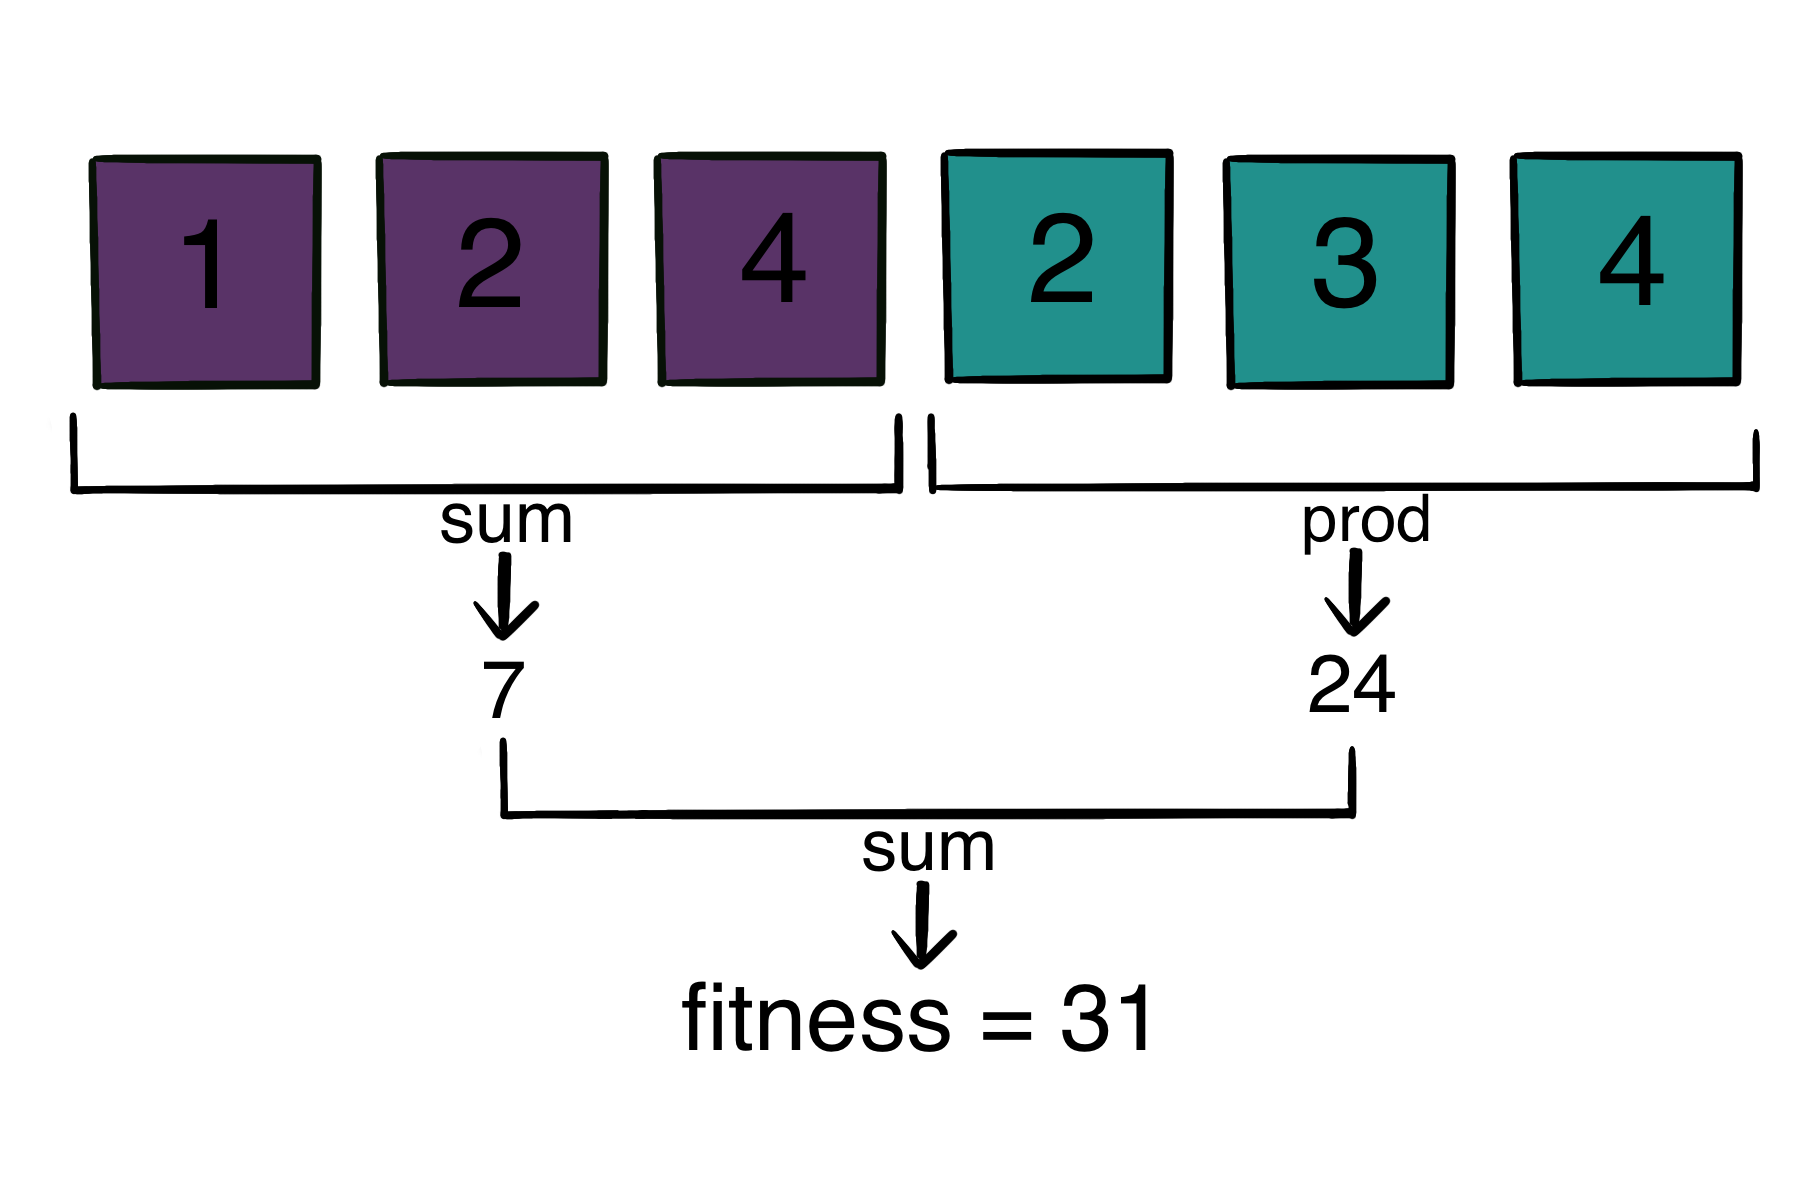
\includegraphics{chapters/1-rank-epistasis/figs/ADDMULT.PNG}
    \caption{Schematic of additive and multiplicative genome for length $n=6$. The first $n/2$ sites are summed and the last $n/2$ sites are multiplied, then the two halves are summed for the final fitness. Image by Katie Gleason.}
    \label{fig:method:admult}
\end{figure}

In this case, the genome was a vector of length $n=20$ of integers between 1 and 4, inclusive (see Fig~\ref{fig:method:admult}). The first 10 integers are summed together, and the last 10 values are multiplied together. The total fitness is the sum of these two values. None of these sites interact epistatically; changing a single site does not affect the fitness contributions of any of the other sites. However, under a baseline assumption that sites should be additive, mutations in the sites which multiply together will appear to create a larger than expected fitness effect. The reverse is true for a baseline assumption of multiplicativity when evaluating the additive sites; they will appear to create a smaller than expected fitnesse ffect. Therefore, we expect traditional metrics which take a baseline for the entire genome to incorrectly identify positive epistasis (under an additive model) or negative epistasis (under a multiplicative model). We therefore compared rank epistasis with the metric $\epsilon$, which has both an additive and multiplicative form \citep{ostman_impact_2011}. 

\subsection{Proof of Concept Experiments}



A good epistasis metric should be able to distinguish between different degrees of epistasis. To confirm that rank epistasis can achieve this goal, we tested it on a landscape where the true degree of interactivity at each site could be calculated.
We used Kauffman NK landscapes \citep{kauffman_towards_1987} for this purpose.
NK landscapes are commonly used epistatic models because they are \textit{tunably rugged}: in NK landscapes, \textit{N} refers to the number of sites in the genome while \textit{K} refers to the number of sites each site interacts with.
Therefore, we can tune how interactive (i.e. how epistatic) the genome is by changing the parameter $K$. 

We tested our metric on a canonical NK landscape, where all sites have equal $K$, and on two variant NK landscapes, where $K$ varied per site. 

\subsubsection{Canonical NK Landscapes}

The canonical landscape allows us to establish how the rank epistasis metric tracks known degrees of interactivity on different genomes, w
Genomes in this case are bitstrings of length $N=100$.
We then allowed the population to evolve on a given NK landscape for $t=10,000$ generations and selected the most fit individual as a reference genome for the rank epistasis algorithm. 
For our canonical NK landscape, we tested the metric on values $K=0, 1, 2, 4, 8$. 

\subsubsection{Variant NK Landscapes}

The variant landscapes allow us to establish how it tracks different degrees of interactivity within the same genome.
As with the canonical landscape, genomes were bitstrings of lenth $N=100$ which evolved for $t=10,000$ generations, and the most fit individual was selected as the reference genome.
Variant landscapes were tested on all pairwise combinations of $K=0, 1, 2, 4, 8$. 

\paragraph{Variant 1: Half-and-Half}
For the first variant, which we call \textit{half-and-half}, we evaluate the first $50$ sites on one NK landscape and the last $50$ sites on a different landscape. Each landscape is independently generated. This allows us to set a different $K$ for each half of the genome. At the boundary, evaluation wraps around to the genome half with the same $K$ value; e.g., if $K=2$, site $49$ interacts with sites $0$ and $1$, whereas site $100$ interacts with sites $50$ and $51$ (Fig~\ref{fig:method:half}.

\begin{figure}
    \centering
    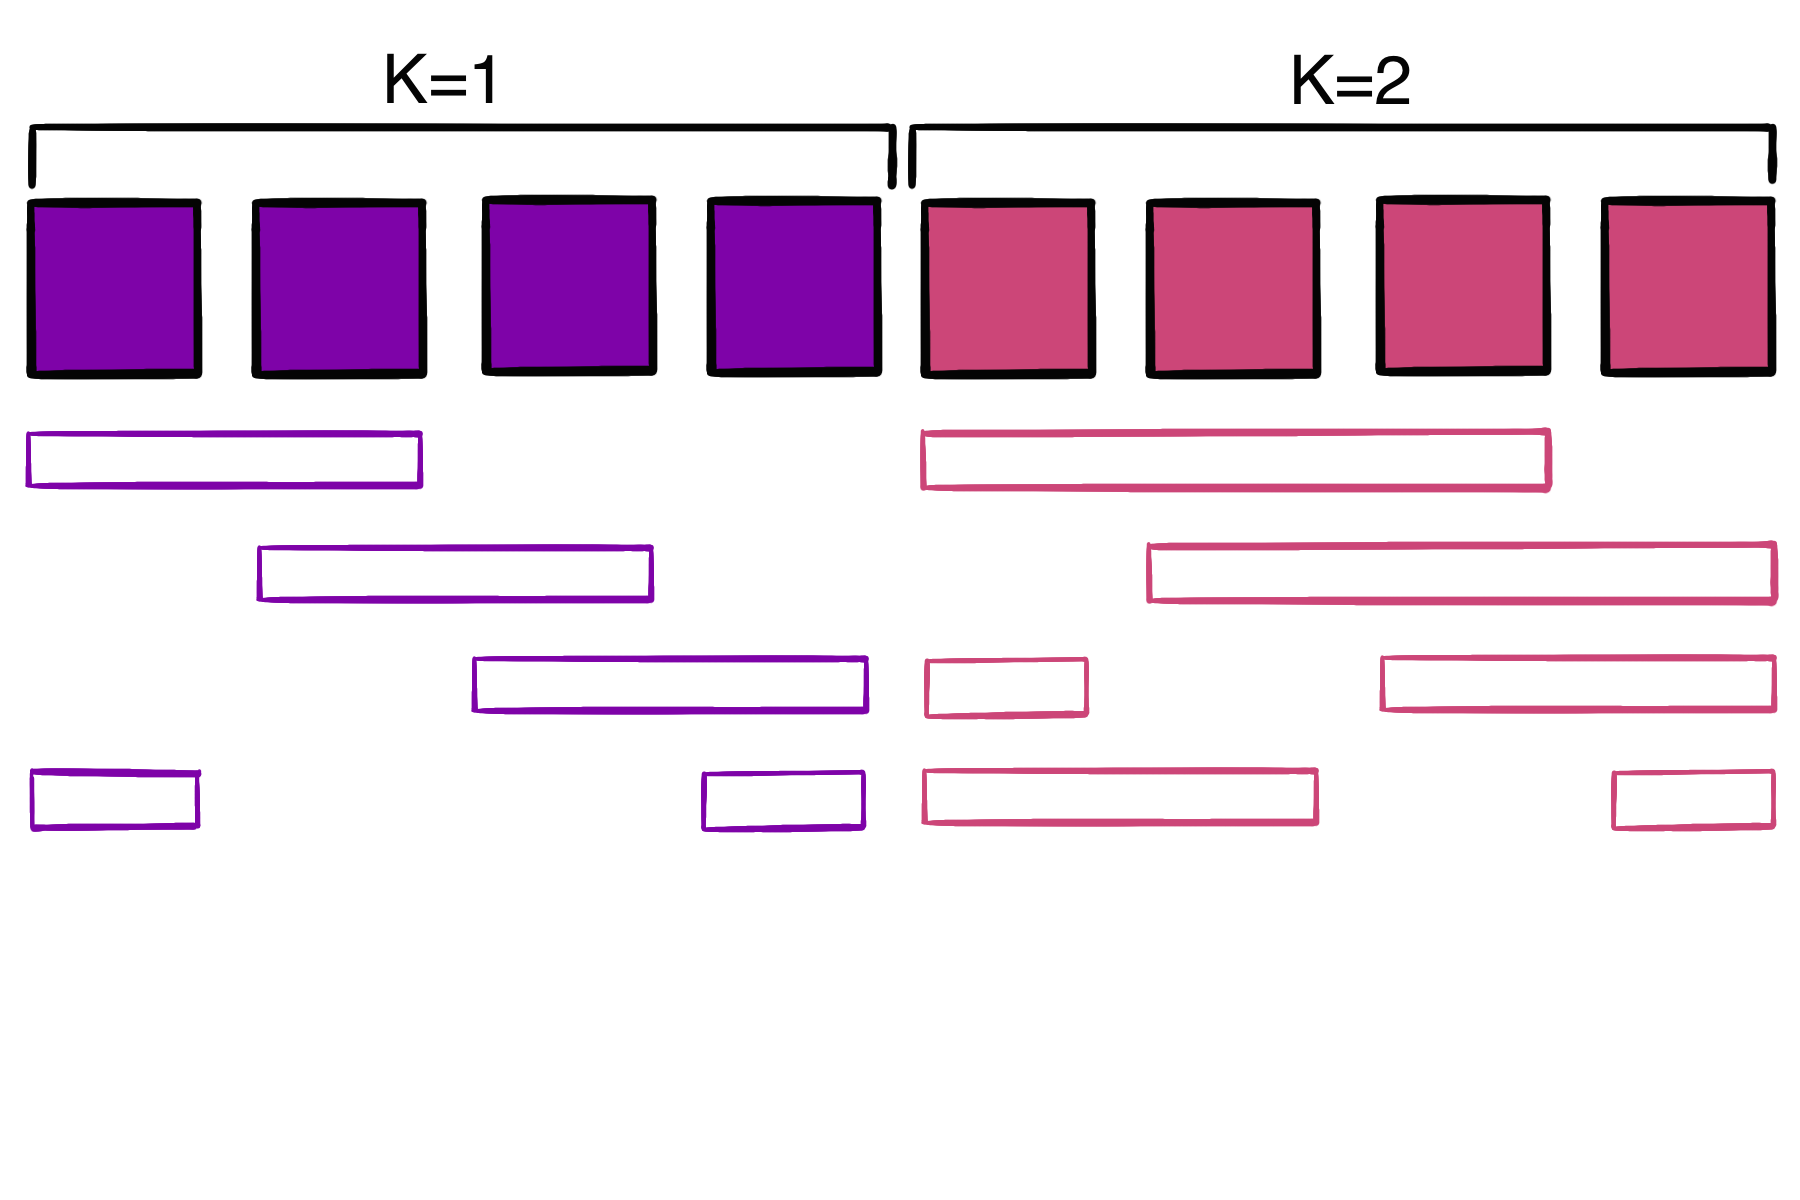
\includegraphics{chapters/1-rank-epistasis/figs/HALF.PNG}
    \caption{Schematic for Half-and-Half landscape with first half $K=1$, second half $K=2$. Filled boxes represent sites of the genome. Empty rectangles underneath are guides for which sites are part of the same evaluation block. Image by Katie Gleason.}
    \label{fig:method:half}
\end{figure}


\paragraph{Variant 2: Mixed}
For the second variant, which we call \textit{mixed}, we evaluate odd-valued sites on one landscape and even-valued sites on a second landscape. Each site still interacts with the adjacent $K$ sites, regardless of odd or even values. In this case, evaluation wraps at the boundary of the genome rather than each landscape. As above, landscapes are independently generated.

\begin{figure}
    \centering
    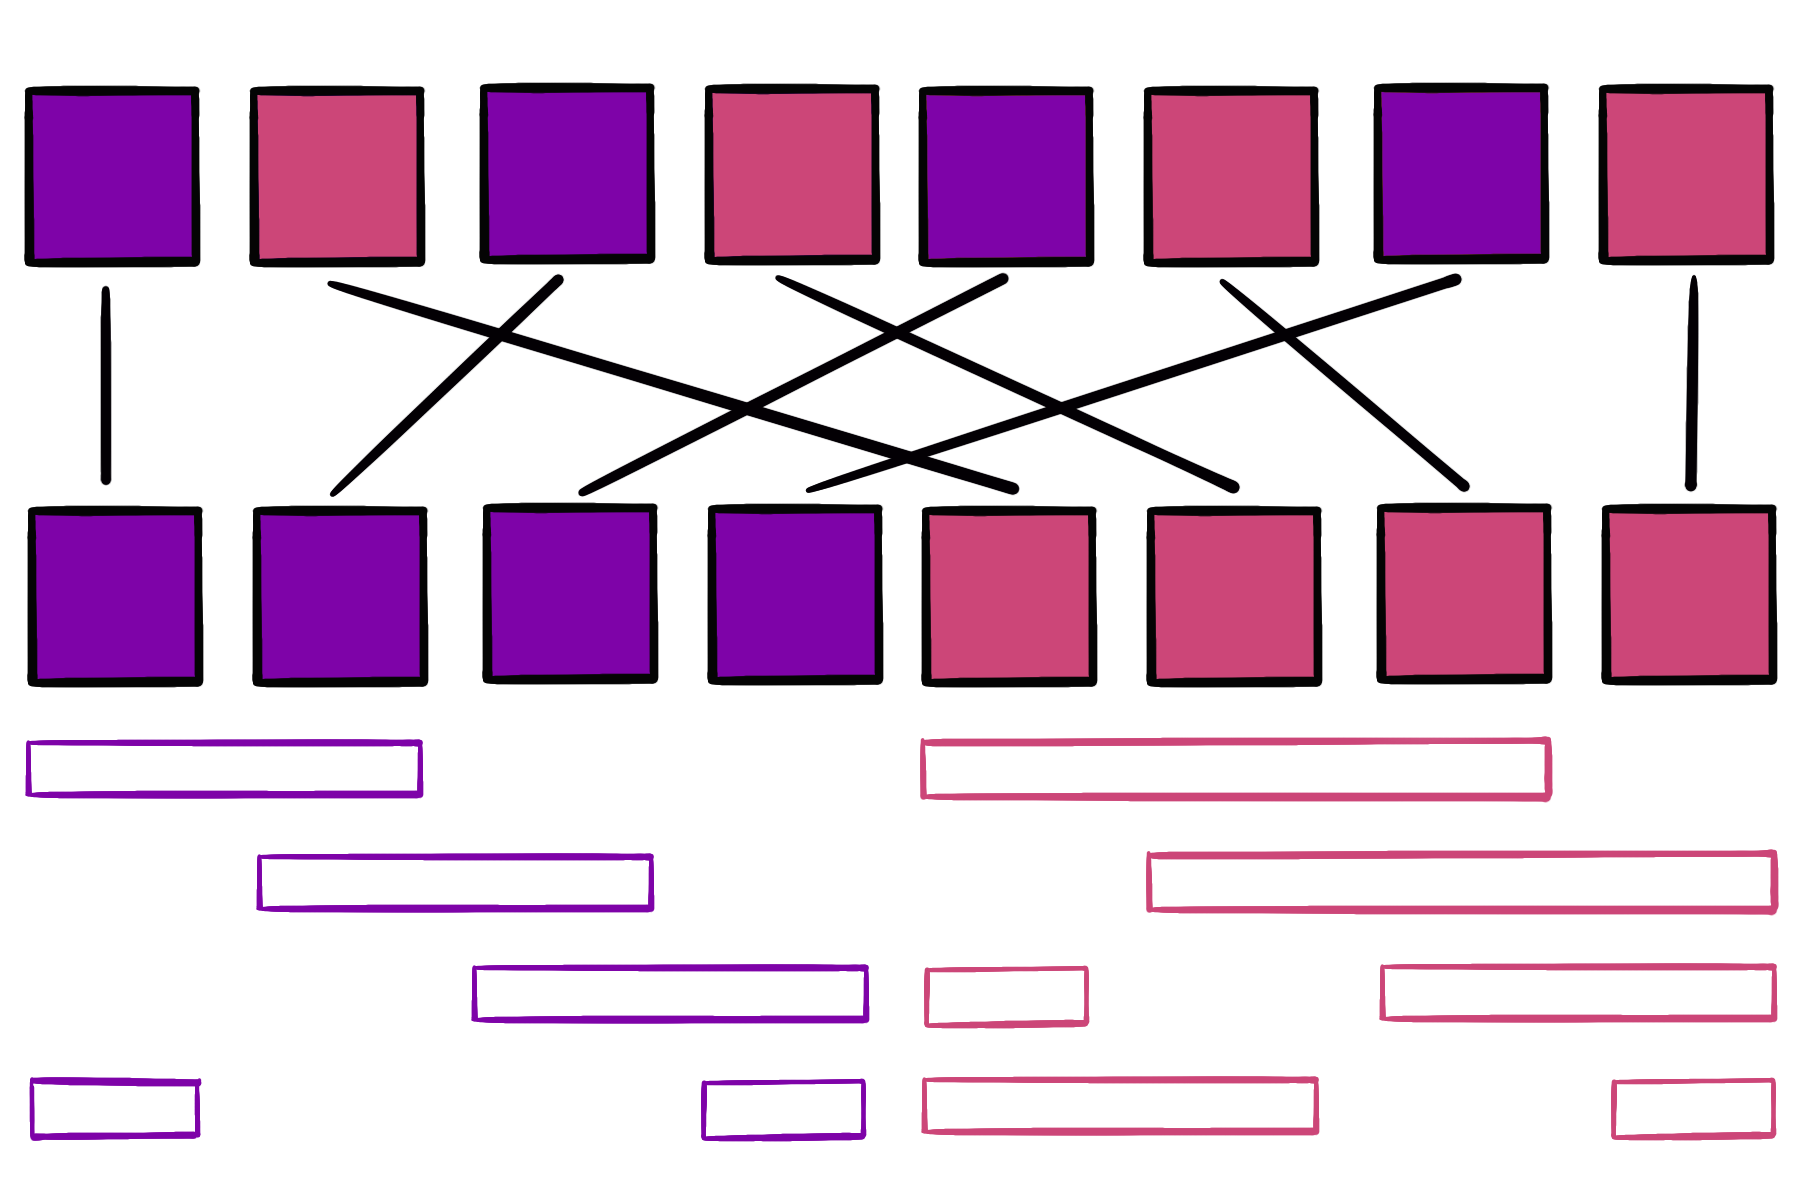
\includegraphics{chapters/1-rank-epistasis/figs/MIXED.PNG}
    \caption{Schematic for Mixed landscape with evens $K=1$, odds $K=2$. Lines indicate how even-valued sites and odd-numbered sites are extracted to form a seperately evaluated genomes. Filled boxes represent sites of the genome. Empty rectangles underneath are guides for which sites are part of the same evaluation block. Image by Katie Gleason.}
    \label{fig:method:half}
\end{figure}


\subsection{Data and Code Availability}

Experiments on the NK landscape were conducted using the Modular Agent-Based Evolver framework (MABE2), an open-source modular digital evolution framework. The source code for MABE2 is available at \url{https://github.com/mercere99/MABE2}. Experiments for the additive and multiplicative comparison were performed in Python (v3.10.4).

Statistical analysis and data visualization was performed in R \citep{r_core_team_r_2019} with the \texttt{tidyverse} library \citep{wickham_welcome_2019}. Implementation of paired Wilcoxon is from \texttt{rstatix} \citep{kassambara_rstatix_2021}.
All data is available at \url{https://doi.org/10.5061/dryad.5dv41ns84}. 
All code for data generation, analysis, and visualization can be found at \url{https://doi.org/10.5281/zenodo.6611759}.